%
% fig-mittelwert.tex -- Abbildung zum Mittelwertsatz
%
% (c) 2026 Prof Dr Andreas Müller
%
\begin{figure}
\centering
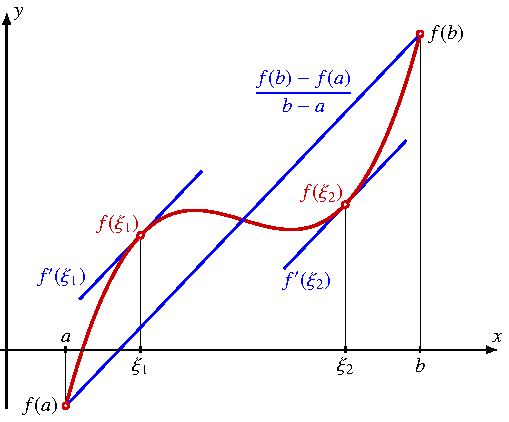
\includegraphics{chapters/020-holomorph/images/mittelwert.pdf}
\caption{Der Mittelwertsatz für eine reelle, differenzierbare Funktion
besagt, dass es zu zwei Werten $a$ und $b$ immer mindestens einen
Zwischenwert $\xi$ gibt, in dem die Steigung von $f(x)$ mit dem
der Sekantensteigung zwischen den Punkten $(a,f(a))$ und $(b,f(b))$
übereinstimmt.
\label{buch:holomorph:fig:mittelwert}}
\end{figure}
